\chapter{On The Design of a Database Management System}
\label{chapter:theory_databases}

\epiquote{Under third normal form, a non-key field must provide a fact about the key, use the whole key, and nothing but the key.}{William Kent}

\acrfull{dbms}, or simply ``databases'', power everything from small and simple websites to large data warehouses that serve millions of users in parallel. Database systems play a crucial role in banking, e-commerce, science, entertainment and practically every aspect of our socio-economic lives, because more and more we rely on insights generated from the analysis of data \cite{Dhar:2013Data} and \acrshort{dbms} form the backbone of many information and data processing systems.

The first commercial \acrshort{dbms} were introduced in the 1960s \cite{Garcia:2009Database} and they have evolved ever since to adapt to a wide range of requirements. Even though many different flavours of \gls{dbms} have emerged over the years, at their core, they still serve the same, fundamental purpose:

\begin{description}
    \item[Management] \acrshort{dbms} enable their users to organize data corpora that can range from a few megabytes to houndreds of terrabytes according to a defined data model. For example, data can be structured into documents \cite{Hashem:2016Evaluating}, graphs \cite{Angles:2008Survey} or tables that in turn can be organized into collections or schemata.
    \item[Definition] \acrshort{dbms} provide users with the ability to alter the organization of their data within the constraints of the data model using a \acrfull{ddl}. 
    \item[Manipulation] \acrshort{dbms} provide users with the ability to modify the data within the constraints of the data model using a \acrfull{dml}. Modifications may include adding, removing or changing entries.
    \item[Querying] \acrshort{dbms} provide users with the ability to query the data using a \acrfull{dql}. Such queries can be used to answer specific ``questions'' about the data and to generate the aforementioned insights.
    \item[Guarantees] \acrshort{dbms} usually provide guarantees, such as assuring durability upon failure or providing access control for concurrent read and write operations. A well-known set of guarantees offered by many modern \acrshort{dbms} is known by its acronym \acrshort{acid} -- which stands for \textbf{A}tomicity, \textbf{C}onsistency, \textbf{I}solation and \textbf{D}urability~\cite{Haerder:1983principles} or \acrshort{base} \cite{Pritchett:2008Base}.
\end{description}

\section{Data Management and Data Models}

\label{section:data_model}

A data model is a formal framework that describes any type of data or information. It usually involves a formal description of the data's \emph{structure}, the \emph{operations} that can be performed and the \emph{constraints} that should be imposed on the data~\cite{Garcia:2009Database}. The purpose of any data model is to formalize how data governed by it can be accessed, modified and queried and any given \acrshort{dbms} usually adopts a specific type of data model (or multiple models, for that matter).


\begin{figure}[b]
    \centering
    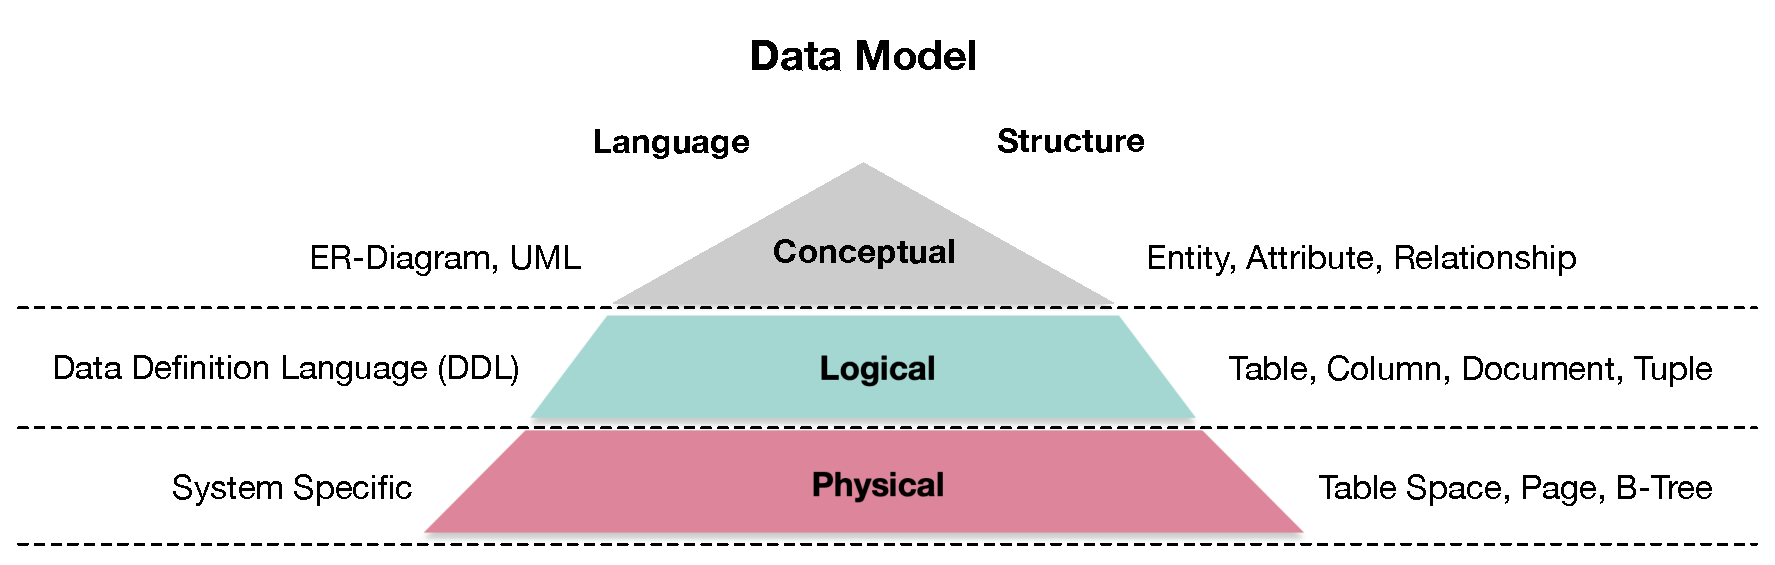
\includegraphics[width=\textwidth]{figures/datamodel_hierarchy.eps}
    \caption{Different levels of abstraction for data modelling.}
    \label{figure:datamodel_hierarchy}
\end{figure}

In the context of database systems and data management, it has become common practice to distinguish between different levels of abstraction for data models, as can be seen in \Cref{figure:datamodel_hierarchy}. At the top, there is the \emph{conceptual data model}, which is often closely tied to some real-world object, fact or process. For example, in an online shop, one can think in terms of customers that place orders, products that are being sold and invoices that must be sent out. In the \acrfull{erm}~\cite{Chen:1976The} -- a popular framework used to describe conceptual data models -- those ``real things'' would be modeled as \emph{entities} that come with \emph{attributes} that describe them and that have \emph{relationships} among them as required by the concrete application.

The \emph{logical data model} is more closely tied to the type of database being used. Different data models have been conceived over the years, including, but not limited to models centered around documents \cite{Hashem:2016Evaluating}, graphs \cite{Angles:2008Survey}, key-value pairs and tables, each bringing the own (often domain-specific) advantages and disadvantages. At this level, one can use \acrshort{ddl} to describe and modify the data organization and \acrshort{dql} or \acrshort{dml} to query and modify the data itself. As an example, one could store each entity described before in a dedicated table wherein each attribute occupies a different column. This is known as the relational data model \cite{Codd:1970Relational} and a very important database language for the relational model would be the \acrfull{sql}, which became an international standard in 1987 under \emph{ISO 9075} and has evolved ever since~\cite{Chamberlin:2012Early}.

At the very bottom, we usually find the \emph{physical data model}, which is specific to the database implementation and describes low-level aspects such data access in terms of \emph{read} and \emph{write} operations to data structures such as \emph{table spaces}, \emph{data pages} or \emph{trees}. An important argument in favour of separating logical from physical data model, even though they are both somewhat specific to a \acrshort{dbms} implementation, is that the end-users should not concern themselves with how exactly data is organized and accessed at the lowest level but should instead describe their intent in terms of the information they are trying to access. Mapping this user-intent to low-level data access operations is then a task of the \acrshort{dbms}.

\section{The Relational Data Model}
\label{section:relational_data_model}

In June 1970, E. F. Codd published his pivotal research article \emph{Relational Model of Data for Large Shared Data Banks}~\cite{Codd:1970Relational} in which he describes a logical data model, which he himself refers to as ``relational''. This model has become the fundament on which many modern database management systems have been built, with examples dating back to the 1970s \cite{Astrahan:1976Systemr} and promintent, contemporary examples include systems such as \emph{Maria DB}, \emph{PostgreSQL} or \emph{Oracle}. 

The relational model is structured around \emph{relations}, which are a mathematical construct but can be visualized as two-dimensional tables. Such a table consists of columns -- which are called \emph{attributes} -- and rows -- which are called \emph{tuples} and hold \emph{attribute values}. Semantically, a relation can be seen as a knowledge-base about some fact -- such as, the paintings held by a museum -- under a \gls{cwa}{}\todo{Reference}. That is, the relation contains all the information available about the fact and can thus be used do derive conclusive answers or results given a stated question or query.

In order to formalize the structure of and the operations that can be executed on the data represented by a relation, one can use \Cref{definition:relation}. 

\begin{definition}[label=definition:relation]{Relation according to \cite{Codd:1970Relational}}{}
    Let $\domain_j$ be sets we call \emph{data domains} with $j \in \left[ 1, N \right]$ and $N \in \symnatural_{> 0}$ . A \emph{relation} $\relation$ constructed over these data domains is a set of $M$ \emph{tuples} $t_i = (a_{i,1}, a_{i,2} ... a_{i,N})$ with $i \in \left[ 1, M \right]$ and $M \in \symnatural_{> 0}$ such that the first attribute value of any tuple comes from $\domain_1$, the second from $\domain_2$ and so forth. That is, values $a_{i,1} \in \domain_1, a_{i,2} \in \domain_2 ... a_{i,N} \in \domain_N$. Ergo, a relation can be seen as a subset of the cartesian product of all data domains over which it was constructed, i.e., $\relation \subset \domain_1 \times \domain_2 ... \times \domain_N$.
\end{definition}

The number of data domains $N$ is referred to as its \emph{degree} and we call such a relation \emph{N-ary}. The number of tuples $M$ is called the \emph{cardinality} of $\relation$ with $M = |\relation|$. It must be noted, that the relational model does not dictate what the data domains $\domain$ are (apart from the constraint that its values must be atomic). However, in a relational \acrshort{dbms}, the they usually correspond to the data types supported by the database and the programming environment it was written in, for example, integer and floating point numbers or text. In this Thesis, we therefore sometimes use \emph{data domain} synonymous for \emph{data type} \footnote{Strictly speaking, the data domains of a given relation $\relation$ are merely subsets of the sets that represent the respective data type which, in turn, are subsets of even more basic sets such as $\symnatural$ or $\symreal$ for \lstinline{Int} and \lstinline{Float} respectively. The relationship between types and data domains is subject of a more categorical approach to data models and nicely layed out in \cite{Spivak:2009Simplicial}}.

In addition to \Cref{definition:relation}, we will use the identities \ref{definition:rel_attribute} to \ref{definition:rel_domains}.

\begin{definition}[label=definition:rel_attribute]{Attributes of a Relation}{}
    Let $\relation$ be a $N$-ary relation over the data domains $\domain_i, \: i \in \left[1, N \right]$ with corresponding names or indexes $l_i$. We call the combination of a data domain with a human readable label \emph{attribute}, that is, $\attribute_{i} = (\domain_i, l_i)$. To simplify notation, we sometimes use the label of an attribute in the subscript instead of the index.
\end{definition}

\begin{definition}[label=definition:rel_schema]{Schema of a Relation}{}
    Let $\relation$ be a $N$-ary relation over the attributes $\attribute_i, \: i \in \left[1, N \right]$. We call the list of all attributes over which $\relation$ was constructed the \emph{heading} or \emph{schema} $\schema (\relation)$ of $\relation$.

    \begin{equation*}
        \schema (\relation) = \left( \attribute \colon \textrm{if} \: \attribute \: \textrm{is an attribute of} \: \relation \right)
    \end{equation*}   
\end{definition}

\begin{definition}[label=definition:rel_attribute_value]{Accessing Attribute Values}{}
    Let $\relation$ be a $N$-ary relation over attributes $\attribute_i, \: i \in \left[1, N \right]$ and let further $t \in \relation$. To address the attribute value $a_i \in t$ that belongs to attribute $\attribute_i \in \schema(\relation) $, we use the \emph{attribute value accessor} $t\left[ \attribute_i \right]$.

    \begin{equation*}
        a_i = t\left[ \attribute_i \right] = \{ a_j \in t \colon i = j \}
    \end{equation*}  
\end{definition}

\begin{definition}[label=definition:rel_domains]{Supported Data Domains}{}
    For a given \acrshort{dbms}, we call $\mathbb{D}$ the set system of data domains or data types supported by the system.
    \begin{equation*}
        \mathbb{D} = \{ \domain \colon \textrm{if} \: \domain \: \textrm{is supported by DBMS} \}
    \end{equation*}
\end{definition}

In its original form, the relational model assumes the following properties to be true for a relation $\relation$ and its attributes~\cite{Codd:1970Relational}:

\begin{description}
    \item[Ordering of Tuples] Tuples $t \in \relation$ are inherently unordered and two relations are considered equal if they contain the same tuples, regardless of order.
    \item[Ordering of Attributes] Attribute values $a_{i}$ always occur in the same order within the tuple $t \in \relation$, which corresponds to the order of the attributes $\attribute_i \in \schema(\relation)$. This order can evolve over time but remains constant in a momentary snapshot of $\relation$. It follows from the definition that $|t| = |\schema(\relation)| \forall t \in \relation$
    \item[Duplicates] Since relations are sets, they do not allow for duplicates, i.e., every tuple $t \in \relation$ must be unique in terms of their attribute values.
\end{description}

Given the idea of a relation, the sum of all data managed by a \acrshort{dbms} can logically be regarded as a collection of different relations $\relation_k, \: k \in \symnatural_{\geq 0}$ of assorted degrees $N_k$ over data domains $\domain \in \mathbb{D}_{\mathtt{dbms}}$ (i.e., a collection of tables). The schema of a database can then be seen as the set system of all $\schema(\relation_k)$. As \cite{Codd:1970Relational} points out, relations are subject to change over time. These changes can take place on the level of any relation's structure, i.e., $\schema(\relation_k)$, the relations $\relation_k$ itself, e.g., by tuples being added to (insert) or removed from (delete) a relation or the level of a tuple $t \in \relation_k$, e.g., by altering one or multiple attribute values.

\cref{example:relational_table} features an example relation $\mathtt{paintings}$ visualized as a table. Each entry in the table represents a painting and the related attribute values.

\begin{example}[label=example:relational_table]{Table Representation of a Relation $\relation_{\mathtt{paintings}}$}{}
    
    The following table lists the content of a ternary relation ($N = 3$) $\relation_{\mathtt{paintings}}$. The attributes $\attribute_{\mathtt{title}}, \attribute_{\mathtt{artist}}, \attribute_{\mathtt{painted}}$ correspond to the table's columns. The individual tuples $\tuple_i$ are ``valid'' combinations of painting title, artist and year of conception under \acrshort{cwa} and constitute the rows.
        
    \begin{center}
        \begin{tabular}{ l || l | l | l |}
            $\relation_{\mathtt{paintings}}$ & $\attribute_\mathtt{title}$  & $\attribute_{\mathtt{artist}}$  & $\attribute_{\mathtt{painted}}$ \\ 
            \hline
            \hline
            $t_1$ & Mona Lisa &  Leonardo da Vinci & 1506 \\
            \hline
            $t_2$ & The Starry Night & Vincent van Gogh & 1889 \\
            \hline
            $t_3$ & Las Meninas & Diego Velázquez & 1665 \\
            \hline
        \end{tabular}
    \end{center}
\end{example}


\subsection{Keys and Normal Forms}

The notion of a relation provides us with the basic tools for data modeling. In addition to \Cref{definition:relation}, Codd proposed a range of constraints to guarantee proper data definition using the relational model and the following constructs~\cite{Codd:1970Relational}:

\begin{description}
    \item[A \acrfull{pk}] $\mathcal{P}$ of relation $\relation$ is a subset of attributes $\mathcal{P} \subset \schema(\relation)$ that uniquely identify a tuple $t \in \relation$. That is, the attributes that are not part of the \acrshort{pk} and the associated values are functionally determined by $\mathcal{P}$. Using \Cref{example:relational_table_pkfk}, the painting and all its attributes, i.e., the artist and the year of its creation, are functionally determined by the name of the painting, which is assumed to uniquely identify the entry.
 
    \item[A \acrfull{fk}] $\mathcal{F}$ of relation $\relation$ is a subset of attributes $\mathcal{F} \subset \schema(\relation)$ that are not member of a \acrshort{pk}, i.e., $ \mathcal{F} \cap \mathcal{P} = \emptyset$, but reference the \acrshort{pk} of $\relation$ or some other relation $R^{*}$. \acrshort{fk} can be used to model relationships between relations. Using \Cref{example:relational_table_pkfk}, the artist that created a painting is referenced through a \acrshort{fk} $\attributef_{\mathtt{artist}}$ in $\relation_{\mathtt{painting}}$ that references the \acrshort{pk} $\attributep_{\mathtt{artist}}$ in $\relation_{\mathtt{artist}}$.
\end{description}

An example of relations with primary and foreign key attributes is given in \cref{example:relational_table_pkfk}. \acrshort{pk}s and \acrshort{fk}s are indicated with star and overline respectively. Note, that we assume here that people (artists) and paintings are uniquely identified by their first and lastname and their title respectively, which is obviously a simplification. In reald-world applications, often artificial \acrshort{pk}s are being generated to avoid unintended collisions. Furthermore, it is typically the task of the \acrshort{dbms} to guarantee entity and referential integrity as part of keeping the data consistent.

\begin{example}[label=example:relational_table_pkfk]{Relations with Primary and Foreign Keys}{}
    
    The following tables lists the schema and extent of $\relation_{\mathtt{paintings}}$ and $\relation_{\mathtt{artists}}$.
    \begin{center}
        \begin{tabular}{ l || l | l | l |}
            $\relation_{\mathtt{painting}}$ & $\attributep_{\mathtt{title}}$  & $\attributef_{\mathtt{artist}}$  & $\attribute_{\mathtt{painted}}$ \\ 
            \hline
            \hline
            $t_1$ & Mona Lisa &  Leonardo da Vinci & 1506 \\
            \hline
            $t_2$ & The Starry Night & Vincent van Gogh & 1889 \\
            \hline
            $t_3$ & Las Meninas & Diego Velázquez & 1665 \\
            \hline
        \end{tabular}
    \end{center}

    \begin{center}
        \begin{tabular}{ l || l | l | l |}
            $\relation_{\mathtt{artist}}$ & $\attributep_{\mathtt{artist}}$ & $\attribute_{\mathtt{birth}}$ & $\attribute_{\mathtt{death}}$\\ 
            \hline
            \hline
            $t_1$ & Leonardo da Vinci & 1452 & 1519 \\
            \hline
            $t_2$ & Vincent van Gogh & 1853 & 1890 \\
            \hline
            $t_3$ & Diego Velázquez & 1599 & 1660 \\
            \hline
        \end{tabular}
    \end{center}
\end{example}

Given the notion of primary and foreign keys, Codd proposed a series of \emph{normal forms} that are an indication of the quality of a data model based on the functional dependency of the attributes on a \acrshort{pk}. The basic idea is to avoid redundancy by normalization, i.e., by putting data that belongs together into dedicated relations and modeling relationships between them using foreign keys. The first three normal forms are as follows:

\begin{description}
    \item[\acrfull{1nf}] requires, that no attribute in a relation has other relations as values, i.e., attributes are atomic and instead, relationships can be established by means of \acrshort{fk}s. Given $\relation_{\mathtt{painting}}$ in \Cref{example:relational_table_pkfk}, this means that $\relation_{\mathtt{artist}}$ cannot be stored as an attribute of $\relation_{\mathtt{painting}}$ (which would be possible according to \Cref{definition:relation}, since data domains can hold any type of element) and instead requires a dedicated relation.
    \item[\acrfull{2nf}] requires, that every non-prime attribute is functionally determined by the whole primary key and not any subset thereof. Given $\relation_{\mathtt{artist}}$ in \Cref{example:relational_table_pkfk} and assuming that  $\attributep_{\mathtt{artist}}$ was split into two attributes $\attributep_{\mathtt{firstname}}$ and $\attributep_{\mathtt{lastname}}$ (composite key), this means that all of the non-prime attributes must be determined by $\attributep_{\mathtt{firstname}}$ and $\attributep_{\mathtt{lastname}}$ jointly, i.e., the full name, and not just either $\attributep_{\mathtt{firstname}}$ or $\attributep_{\mathtt{lastname}}$.
    \item[\acrfull{3nf}] requires, that every non-prime attribute is functionally determined solely by the primary key and that they do not depend on any other attribute. Given $\relation_{\mathtt{artist}}$ in \Cref{example:relational_table_pkfk}, this means that all of the non-prime attributes must be determined by $\attributep_{\mathtt{artist}}$ alone.
\end{description}

All the normal forms build onto one another, i.e., for a data model to be considered \acrshort{3nf} is also required to satisfy \acrshort{2nf}  and \acrshort{1nf}\footnote{This has led to the mnemonic \emph{``The key, the whole key, and nothing but the key, So help me Codd.''} in reference to a similarly structured oath often used in courts of law.}. Additional normal forms up to \emph{6NF} and the \acrfull{bcnf}, a slightly stronger version of \acrshort{3nf}, have been defined. For the sake of brevity, we will ommit those since they are not relevant for the discussion ahead.

\subsection{Relational Algebra}
\label{section:rel_algebra}

Having introduced the aspect of data representation and constraints, we can now move to that of operations that can be performed on the data upon querying. For that purpose, \cite{Codd:1970Relational} proposed the idea of a \emph{relational algebra}, which follows a simple yet powerful idea: All query operations performed on relations are expressed by a set of \emph{relational operators} that take one or multiple relations as input and output a new relation as expressed by \Cref{equation:rel_op}.

\begin{equation}
    \label{equation:rel_op}
    \mathtt{OP}: \relation_1, \ldots, \relation_n \rightarrow \relation_{O}
\end{equation}

Those relational operators can then be composed to express a query of arbitrary complexity as indicated by \Cref{equation:rel_query}.

\begin{equation}
    \label{equation:rel_query}
    \mathtt{QUERY} = \mathtt{OP_{1}} \circ \mathtt{OP_{2}}, \ldots , \circ \mathtt{OP_{m}}
\end{equation}

In addition to this idea, Codd proposed a minimal set of relational operators listed in \Cref{table:relational_operators} and explained in the following sections. For the sake of completeness, it must be mentioned that notation and operators may slightly differ depending on the literature. We mainly use \cite{Garcia:2009Database} as our reference, with a few adjustments of our own for the sake of internal consistency.

\begin{table}
    \caption{The relational operators proposed by Codd et al. \cite{Codd:1970Relational,Garcia:2009Database}.}
    \label{table:relational_operators}
    \begin{tabular}{| l | c | c | p{75mm} |}
        \hline
       \textbf{Name} & \textbf{Symbol} & \textbf{Arity}  & \textbf{Example} \\ 
        \hline
        \hline
        Union & $\cup$  & 2 & Set union of two input relations. \\
        \hline
        Intersection & $\cap$  & 2 & Set intersection of two input relations. \\
        \hline
        Difference & $\setminus$  & 2 & Set difference of two input relations. \\
        \hline
        Cartesian Product & $\times$ & 2 & Pairs each tuple from one the left with every tuple of the right input relation and concatenates them. \\
        \hline
        Rename & $\rho_{\attribute_\mathtt{A} \rightarrow \attribute_\mathtt{B}}$ &  1 & Renames attribute $\attribute_\mathtt{A}$ in input relation to $\attribute_\mathtt{B}$. \\
        \hline
        Selection & $\selection_{\mathcal{P}}$ &  1 & Removes tuples from the input relation that don't match predicate $\mathcal{P}$. \\
        \hline
        Projection & $\projection_{\chi}$ &  1 & Removes attributes from the input relation that are not included in $\chi$. \\
        \hline
        Natural join & $\Join_{\mathcal{P}}$ & 2 & Pairs each tuple from the left with every tuple of the right input relation if their shared attributes match and concatenates them. \\
        \hline
    \end{tabular}
\end{table}

\subsubsection{Simple Set Operations}

Since relations are in essence sets of tuples, all basic operations known from set theory can be applied, namely \emph{union}, \emph{intersection} and \emph{difference}, with the only constraint that the two input relations $\relation_L,\relation_R$ must be \emph{union compatible} and thus exhibit the same attributes, i.e., $\schema(\relation_L) = \schema(\relation_R)$.

The set union $\relation_L \cup \relation_R$ generates a new relation of all tuples contained in either $\relation_L$ OR $\relation_R$, as expressed by \Cref{equation:rel_op_union}. Due to relations being sets, duplicates resulting from a union operation are \emph{implictly} eliminated.

\begin{equation}
    \label{equation:rel_op_union}
    \relation_L \cup \relation_R = \{ t \colon t \in \relation_L \symor t \in \relation_R \}
\end{equation}

The intersection $\relation_L \cap \relation_R$ generates a new relation of all tuples contained in $\relation_L$ AND $\relation_R$, as expressed by \Cref{equation:rel_op_intersection}.

\begin{equation}
    \label{equation:rel_op_intersection}
    \relation_L \cap \relation_R = \{ t \colon t \in \relation_L \symand t \in \relation_R \}
\end{equation}

The difference $\relation_L \setminus \relation_R$ generates a new relation of all tuples contained in $\relation_L$ AND NOT in $\relation_R$, as expressed by \Cref{equation:rel_op_difference}.

\begin{equation}
    \label{equation:rel_op_difference}
    \relation_L \setminus \relation_R = \{ t \colon t \in \relation_L \symand t \notin \relation_R \}
\end{equation}

These basic set operations simply combine two input relations without changing its structure, i.e., $\schema(R_{L}) = \schema(R_{R}) =  \schema(R_{O})$. 

\subsubsection{Cartesian Product}
The binary, \emph{cartesian product} or \emph{cross product} $\relation_L \times \relation_R$ of two input relations $\relation_L,\relation_R$ concatenates every tuple $t_{L} \in \relation_L$ with every tuple $t_{R} \in \relation_R$ to form a new output tuple, as expressed by \Cref{equation:rel_op_cartesian}.

\begin{equation}
    \label{equation:rel_op_cartesian}
    \relation_L \times \relation_R = \{ (t_L, t_R) : t_L \in \relation_L \wedge t_R \in \relation_R \}
\end{equation}

The result is a relation that contains all the attributes of $\relation_L$ and $\relation_R$, i.e., $\schema(\relation_L \times \relation_R) = \schema(\relation_L) \cup \schema(\relation_R)$ and every possible permutation of tuples from the input relations.

\subsubsection{Rename}
The unary \emph{rename} operator $\rho_{\attribute_\mathtt{A} \rightarrow \attribute_\mathtt{B}}(\relation)$ renames the attribute $\attribute_\mathtt{A}$ to $\attribute_\mathtt{B}$ without changing any value. This can be useful to elliminate collisions before applying the cartesian product or to enable a natural join on differently named attributes.

\subsubsection{Selection}

The unary, generalized \emph{selection} operator $\selection_{\phi}(\relation)$ applied on an input relation $\relation$ creates an output relation that contains a subset of tuples $t \in \relation$ such that only tuples that match the predicate $\phi$ are retained as expressed by \Cref{equation:rel_op_selection}.

\begin{equation}
    \label{equation:rel_op_selection}
    \selection_{\phi}(\relation) = \{ t \in \relation \colon \phi(t) \} \subset \relation
\end{equation}

The predicate $\phi$ can be any conditional statement consisting of individual atoms that involve attributes of $\relation$ or any constant value and comparison operators $=,\neq,>,<,\geq, \leq$. Individual atoms can also be combined by logical operators $\symand$, $\symor$ or $\symnot$. Examples could be $\attribute_1 \geq 2$, $\attribute_2 = \attribute_3$ or $\attribute_1 \geq 2 \wedge \attribute_2 = \attribute_3$ to express that an attribute should be greater than a constant, equal to another attribute or combine the two with $A_1,A_2,A_3 \in \schema(\relation)$.


\subsubsection{Projection}
The unary \emph{projection} operator $\projection_{\chi}(\relation)$ with $\chi \subset \schema(\relation)$ applied on an input relation $\relation$ creates an output relation that only contains the attributes listed in $\chi$, i.e., $\schema(\projection_{\chi}(\relation)) = \chi$, as expressed by \cref{equation:rel_op_projection}.

\begin{equation}
    \label{equation:rel_op_projection}
    \projection_{\chi}(\relation) = \{ t\left[ \chi \right] : t \in \relation \} \: \textrm{with} \: t\left[ \chi \right] = \{ t[\attribute] \colon \attribute \in \chi \}
\end{equation}

All the tuples in $\relation$ are retained, however, resulting duplicates are removed.

\subsubsection{Natural Join}

The binary, \emph{natural join} operator $\relation_L \Join \relation_R$ on two input relations $\relation_L$, $\relation_R$ concatenates every tuple $t_{L} \in \relation_L$ with every tuple $t_{R} \in \relation_R$ to form a new output tuple, if the attribute values of $t_{L}$ and $t_{R}$ are the same for the shared attribues $\xi = \{ \attribute : \attribute \in \schema(\relation_L) \symand \attribute \in \schema(\relation_R) \}$ as expressed by \Cref{equation:rel_op_join}

\begin{equation}
    \label{equation:rel_op_join}
    \relation_L \Join \relation_R = \{ t_L \cup t_R : t_L \in \relation_L \symand t_R \in \relation_R \symand t_L\left[ \xi \right] = t_R\left[ \xi \right] \}
\end{equation}

The result is a relation that contains all the attributes of $\relation_L$ and $\relation_R$, i.e., $\schema(\relation_L \Join \relation_R) = \schema(\relation_L) \cup \schema(\relation_R)$. Shared attributes are only retained once.

\subsubsection{Expressing Queries}

The following \Cref{example:rel_alg_query} illustrates how relational operators can be combined to form complex queries. Since expressing queries in such a way is quite inconvenient, in practice, queries are usually expressed through an intermediate query language, which is then translated to the relational operators. A famous example of such a language is \acrshort{sql} \cite{Chamberlin:2012Early} for relational databases.

\begin{example}[label=example:rel_alg_query]{Searching for Paintings Using Relational Algebra}{}

    The following tables lists the schema and extent of $\relation_{\mathtt{paintings}}$ and $\relation_{\mathtt{artists}}$.

    \begin{center}
        \begin{tabular}{ l || l | l | l |}
            $\relation_{\mathtt{painting}}$ & $\attributep_{\mathtt{title}}$  & $\attributef_{\mathtt{artist}}$  & $\attribute_{\mathtt{painted}}$ \\ 
            \hline
            \hline
            $t_1$ & Mona Lisa &  Leonardo da Vinci & 1506 \\
            \hline
            $t_2$ & The Starry Night & Vincent van Gogh & 1889 \\
            \hline
            $t_3$ & Las Meninas & Diego Velázquez & 1665 \\
            \hline
        \end{tabular}
    \end{center}

    \begin{center}
        \begin{tabular}{ l || l | l | l |}
            $\relation_{\mathtt{artist}}$ & $\attributep_{\mathtt{artist}}$ & $\attribute_{\mathtt{birth}}$ & $\attribute_{\mathtt{death}}$\\ 
            \hline
            \hline
            $t_1$ & Leonardo da Vinci & 1452 & 1519 \\
            \hline
            $t_2$ & Vincent van Gogh & 1853 & 1890 \\
            \hline
            $t_3$ & Diego Velázquez & 1599 & 1660 \\
            \hline
        \end{tabular}
    \end{center}

    Using relational algebra, the query ``return the names of all paintings that were painted by an artist who died after 1800'' can be expressed by joining $\relation_{\mathtt{paintings}}$ and $\relation_{\mathtt{artists}}$, followed by a selection and projection:

    \begin{equation*}
        \relation_{\mathtt{result}} = \projection_{\attribute_{\mathtt{title}}} (\selection_{\attribute_{\mathtt{death}} \geq 1800}(\relation_{\mathtt{paintings}} \Join \relation_{\mathtt{artists}}))
    \end{equation*}

 This query produces the relation $\relation_{\mathtt{result}}$ that contains $t_2$ of $\relation_{\mathtt{paintings}}$.
\end{example}

\subsection{Extensions}
\label{section:rel_extensions}

While the relational model and its algebra forms the foundation of many modern \glsname{dbms}, the model as originally proposed by Codd has often turned out to be too limited to accomodate certain functionality as required, e.g., by the ANSI \acrshort{sql} standard \cite{Libkin:2003Expressive,XOpen:1996SQL}. For example, many applications require storage of duplicate data and therefore, the notion of a relation -- which is a set of tuples and thus does not allow for duplicates -- is inadequate. Another example could be the support for sorting or aggregation (\texttt{ORDER BY} and \texttt{GROUP BY} in \acrshort{sql}), which also isn't covered by the original algebra.

Over the years, this has led to a growing list of proposals for extensions, some of which have seen adoption while a majority has remained theoretical in nature. In the following sections, we will introduce a few examples. While at a first glance, these adaptions seem to be an elegant way of extending the expressiveness of the relational data model, there are important implications: Most importantly, some operators may not behave in the way specified in \Cref{section:rel_algebra} or we may require additional or different operators to accomodate all the functionality needed. This adds complexity to the \acrshort{dbms}, especially when considering aspects such as query planning.

\subsubsection{Relations vs. Bags vs. Sequences}

The motivation for considering other mathematical structures than sets as an algebraic foundation for a data model are twofold: Firstly, relations are unable to provide functionality that may be desirable in a \acrshort{dbms}, such as duplicate entries or explicit ordering of tuples. Secondly, some of the mathematical convenience of the relational model, e.g., prohibiting duplicates, may be inefficient to actually implement~\cite{Garcia:2009Database}. It is therefore not surprising that ANSI \acrshort{sql}  \cite{XOpen:1996SQL} formally operates on \emph{bags} rather than sets, which allow for duplicate entries \cite{Garcia:2009Database,Chamberlin:2012Early}. If one would want to express explicit ordering of tuples, we could even have to move to sequences, in which every tuple occupies a specific position.

We will not elaborate on all the consequences such a transition may have and refer to \cite{Garcia:2009Database}, which discusses this issue in great detail. However, for illustrative  purposes, we still provide the \Cref{example:bag_vs_set} inspired by \cite{Garcia:2009Database}. It demonstrates that even minor changes to the properties of the purely relational data model must be taken into account when implementing systems, e.g., during algebraic query optimisation.

\begin{example}[label=example:bag_vs_set]{Searching for Paintings Using SQL}{}

    The following tables list the schema and extent of $\relation_{\mathtt{p1}}$ and $\relation_{\mathtt{p2}}$, which are union compatible and have one tuple in common ($t_1$).

    \begin{center}
        \begin{tabular}{ l || l | l | l |}
            $\relation_{\mathtt{p1}}$ & $\attributep_{\mathtt{title}}$  & $\attributef_{\mathtt{artist}}$  & $\attribute_{\mathtt{painted}}$ \\ 
            \hline
            \hline
            $t_1$ & Mona Lisa &  Leonardo da Vinci & 1506 \\
            \hline
            $t_2$ & The Starry Night & Vincent van Gogh & 1889 \\
            \hline
            $t_3$ & Las Meninas & Diego Velázquez & 1665 \\
            \hline
        \end{tabular}
    \end{center}

    \begin{center}
        \begin{tabular}{ l || l | l | l |}
            $\relation_{\mathtt{p2}}$ & $\attributep_{\mathtt{title}}$  & $\attributef_{\mathtt{artist}}$  & $\attribute_{\mathtt{painted}}$ \\ 
            \hline
            \hline
            $t_1$ & Mona Lisa &  Leonardo da Vinci & 1506 \\
            \hline
            $t_2$ & The Birth of Venus & Sandro Botticelli & 1485 \\
            \hline
            $t_3$ & The Night Watch & Rembrandt Harmenszoon van Rijn & 1642 \\
            \hline
        \end{tabular}
    \end{center}
    
    If now we look at the union operator, i.e., $\relation_{p} = \relation_{\mathtt{p1}} \cup \relation_{\mathtt{p2}}$, we will see, that if we consider these to be normal relations, then $|\relation_{p}| = 5$, whereas for bags, $|\relation_{p}| = 6$, since since the common tuple will appear twice.

    Now let us further consider the set difference and the distributive law with union, i.e., $(\relation_{\mathtt{p1}} \cup \relation_{\mathtt{p2}}) \setminus \relation_{\mathtt{p1}} = (\relation_{\mathtt{p1}} \setminus \relation_{\mathtt{p1}}) \cup (\relation_{\mathtt{p2}} \setminus \relation_{\mathtt{p1}})$. We can easily see, that this identity holds for sets but not for bags, since $|(\relation_{\mathtt{p1}} \setminus \relation_{\mathtt{p1}}) \cup (\relation_{\mathtt{p2}} \setminus \relation_{\mathtt{p1}})| = 2$ wheras $|(\relation_{\mathtt{p1}} \cup \relation_{\mathtt{p2}}) \setminus \relation_{\mathtt{p1}}| = 3$, since one of the duplicates will be retained.
\end{example}

\subsubsection{Extended Projection}

The extended project as described by \cite{Garcia:2009Database} is an addition to the projection operator $\projection_{\chi}$ specified in the relational data model and necessitated by the ANSI SQL standard \cite[]{XOpen:1996SQL}. It involves a more general definition of $\chi$, that can now contain any of the following elements for a relation $\relation$ \footnote{We deliberately deviate from \cite{Garcia:2009Database} in that we don't limit ourselves to algebraic expressions and special functions.}:
\begin{enumerate*}[label=(\roman*)]
    \item any attribute $\attribute \in \schema(\relation)$,
    \item any literal value $\mathcal{L} \in \domain_{\mathcal{L}}, \text{ with } \domain_{\mathcal{L}} \in \domainset$ or,
    \item any N-ary function expression $\mathcal{E} \colon \mathcal{G}_1 \times, \ldots, \times \mathcal{G}_A \rightarrow \mathcal{A}_{\text{out}}$ with $\mathcal{G}_j$ being either an attribute $\attribute_i \in \schema(\relation)$ or a literal $\mathcal{L}_j \in \domain_{\mathcal{L}}$.
\end{enumerate*}

Therefore, in addition to projecting on existing attributes, the extended projection can be used to project onto literal values and arbitrary function expressions, thus appending new attributes to a relation. This is a very powerful extension, because it enables the generation of new values based on existing ones. A lot of \acrshort{dbms} also allow users to define their own \acrfull{udf}.

\subsubsection{Aggregation}

Aggregation is the act of summarizing certain attribute values based on the membership of a tuple in a specific category or group, which is established based on other attribute values. An example could be a customer who would like to see the maximum price of all products per brand. The ANSI \acrshort{sql} standard \cite{XOpen:1996SQL} defines the \texttt{GROUP BY} operator for this purpose.

\cite{Garcia:2009Database} formalises the grouping operator $\group_{G}$, which can be used to aggregate on attributes in $\relation$. $G$ is a list of elements, which can either be:
\begin{enumerate*}[label=(\roman*)]
    \item any attribute $\attribute \in \schema(\relation)$, the attribute(s) that the operator aggregates by or,
    \item any aggregation or set function $\texttt{AGR} \colon \mathcal{A} \rightarrow \mathcal{A}_{\text{out}}$
\end{enumerate*}

The output relation $\group_G (\relation)$ is then constructed as follows: First, the tuples in the input relation  $\relation$ are grouped into $N$ groups $\mathcal{G}_1, \ldots,\mathcal{G}_N \subset \relation$ based on the values in the specified grouping attribute(s). Subsequently, the aggregation function is executed for all tuples in each group, giving rise to an output relation that contains $N$ tuples --  one per group -- each bearing the grouping attributes as well as the ouput of the set functions. The ANSI \acrshort{sql} standard \cite{XOpen:1996SQL} defines a list of supported set functions including but not limited to functions such as \texttt{COUNT}, \texttt{MIN}, \texttt{MAX}, \texttt{SUM} and \texttt{MEAN}.

\subsubsection{Sorting and Ranking}

Sorting is the act of arranging items in a specific order based on their attribute values. Consider, for example, a customer who wants to look at prices of products from lowest to highest. The ANSI \acrshort{sql} standard \cite{XOpen:1996SQL} defines the \texttt{ORDER BY} operator for this purpose.

However, formally, the act of sorting is difficult in the context of ``pure'' relational algebra because neither sets nor bags exhibit any ordering. \cite{Garcia:2009Database} proposes the $\order_T$ operator to make this operation explicit. Given a relation $\relation$, $T$ is simply a list of attributes to sort on, i.e., $T \subset \schema(\relation)$ and the result $\order_T (\relation)$ is a sorted list of values. The conversion between set, bag and list takes place implicitly through application of the operator and the consequences for the algebra are not addressed.

More formal approaches to sorting were proposed, e.g., by \cite{Ramakrsihnan:1998SRQL} who introduced four additional operators and a \emph{sequence algebra} that can deal with ordered queries Similarly, \cite{Chengkai:2005RankSQL} proposes a more systematik approach to \emph{ranking}, which is sorting based on an external function. They introduce the idea of a \emph{rank relation}, which carries explicit properties w.r.t to the ranking applied.

\pagebreak

\section{\acrfull{dbms}}
Irrespective of the concrete system and data model, \acrshort{dbms} generally exhibit an internal structure that is very similar \cite{Petrov:2019Database,Hellerstein:2007Architecture} even though, specifics may vary widely between implementions. This overall structure is depicted in \Cref{figure:dbms-architecture} and in this section we use the path a query takes within such a system, as indicated by the directed, red arrows, to illustrate the components involved in its execution.

\begin{figure}[tb]
    \centering
    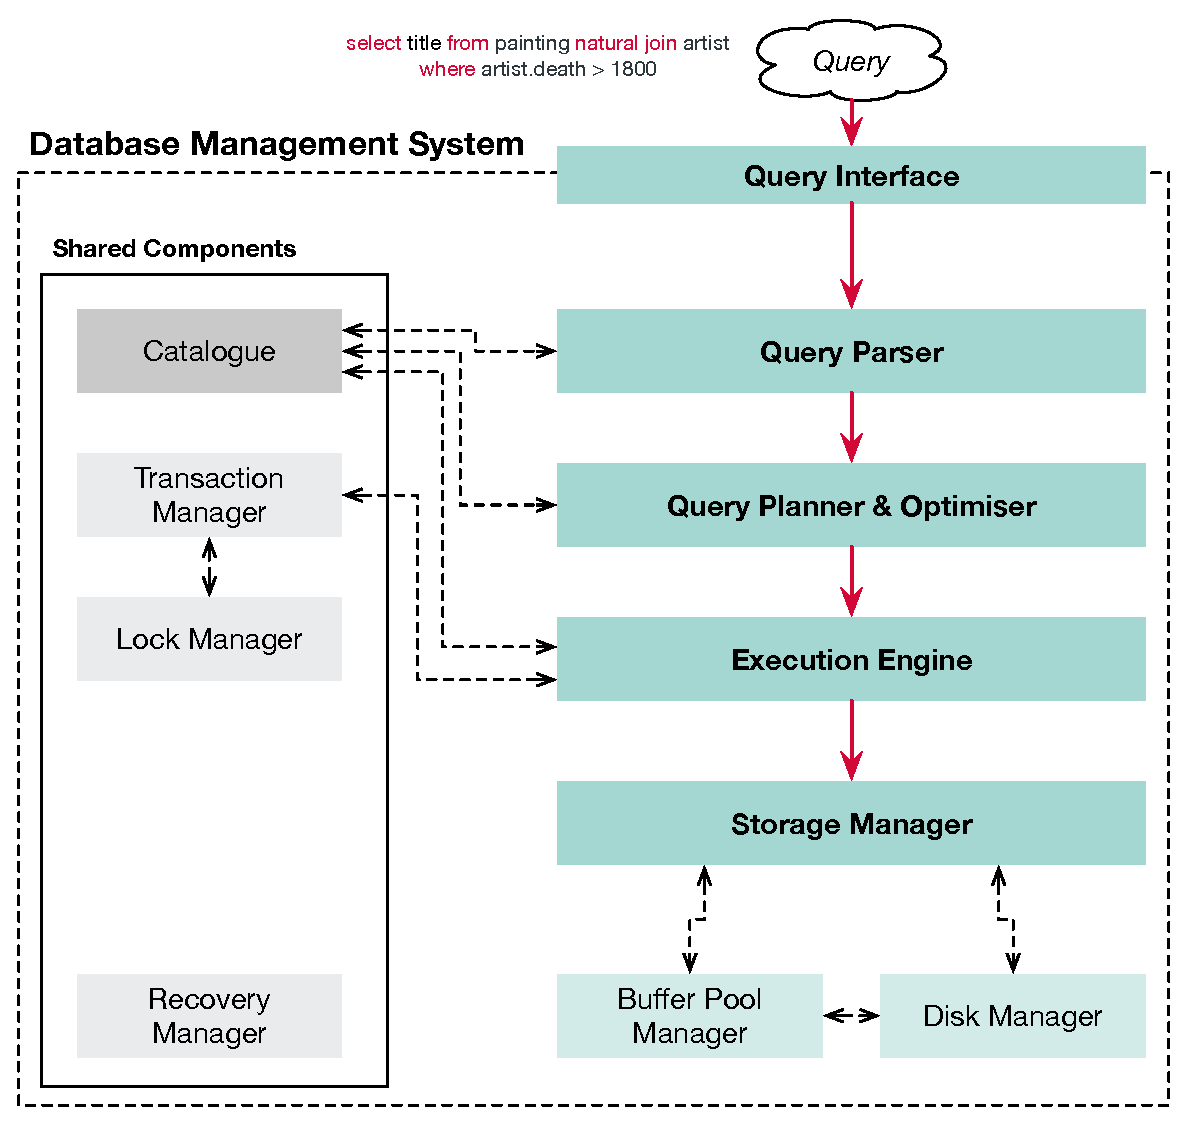
\includegraphics[width=0.95\textwidth]{figures/dbms-architecture.eps}
    \caption{The general architecture of a \acrshort{dbms} and its individual components.}
    \label{figure:dbms-architecture}
\end{figure}

\subsection{Query Interface}

The query interface is the \acrshort{dbms}'s channel to the outside world and enables its use by other systems. The query interface takes care of client connections, accepts and forwards queries into the database and returns results to the caller. Since in modern systems, communication usually takes place over network connections, the query interface must also handle the details of communication.

Queries accepted by the query interface are usually expressed in a specific query language -- which are often designed for human user's and therefore human-readable. We have already mentioned \acrshort{sql} \cite{Chamberlin:2012Early} as the most prominent example of such a query language, which can be used to express queries using a declarative, textual syntax (see \Cref{example:sql_query}). In addition to SQL, there also exist other, domain-specific languages such as SPARQL \cite{Perez:2009Semantics} to query \acrfull{rdf} data, \emph{Cypher} to query labeled property graphs \cite{Francis:2018Cypher} found in graph databases such as \emph{Neo4j} \footnote{https://neo4j.com/} or the document-oriented query language used by \emph{MongoDB} \footnote{https://www.mongodb.com/}.

\begin{example}[label=example:sql_query]{Searching for Paintings Using SQL}{}

    Again using the relations $\relation_{\mathtt{paintings}}$ and $\relation_{\mathtt{artists}}$ from \Cref{example:rel_alg_query}, the query ``return the names of all paintings that were painted by an artist who died after 1800'' can be expressed in \acrshort{sql} as follows \cite{Graefe:1993Query}:

    \begin{lstlisting}[language=SQL, showspaces=false, basicstyle=\ttfamily, numbers=left, numberstyle=\tiny]
        select * from paintings natural join artists where artist.death > 1800
    \end{lstlisting}

    The \texttt{select} clause expresses the projection $\projection$ to all attributes (*), the \texttt{natural join} clause expresses the natural join $\Join$ between \texttt{paintings} \& \texttt{artist} and the \texttt{where} clause expresses the selection $\selection$ to tuples whose \texttt{artist.death} attribute is greater than 1800.
\end{example}

Early attempts at a client-facing standardisation of the query interface for SQL-based systems led to the inception of the \acrfull{cli} standard \cite{XOpen:1995CLI}, which in its early version enabled embedding of \acrshort{sql} commands into C or Cobol programms. The \acrshort{cli} standard was later complemented by \acrfull{odbc} and \acrfull{jdbc}, which provide database connectivity to a wide range of \acrshort{sql} and NoSQL systems. In addition, most of the SQL (e.g., MySQL, PostgreSQL, MS-SQL, Oracle) and NoSQL (e.g., MongoDB, Neo4j, Redis) provide database specific and therefore un-standardised connectivity thorugh a plethora of client libraries that are maintained for different platforms and programming environments by either companies and / or open source contributors.

\subsection{Query Parser}

The query parser's main task is to transform a query provided in a human-readable query language to a logical representation that can be processed by a \acrshort{dbms}. This often involves a conversion of a syntax to the operators specified by the data model, e.g., a tree of the relational operators that represent an \acrshort{sql} query (see \Cref{figure:query-tree}, for example). The result is what is generally called a \emph{logical query (execution) plan}, since it outlines all the operations necessary to generate the desired results without, however, specifying concrete access methods or algorithms.

\begin{figure}[tb]
    \centering
    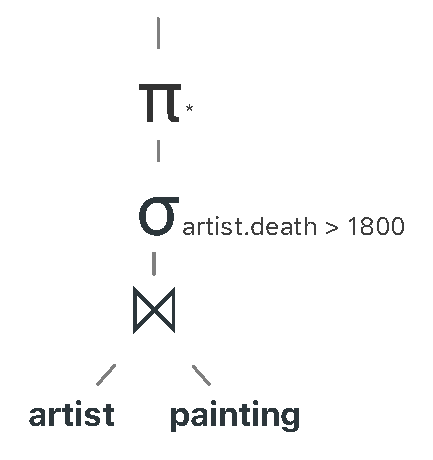
\includegraphics[width=\textwidth]{figures/query-tree.eps}
    \caption{The query from \Cref{example:sql_query} represented as a tree of relational opertors also called a logical query execution plan. By convention, the tree is executed and read from left to right (bottom to top) and information flows from the leafs to the root.}
    \label{figure:query-tree}
\end{figure}

Practically, query parsing involves several steps \cite{Graefe:1993Query,Garcia:2009Database}: First, the syntax of the textual query must be analysed and converted to a data structure that can be processed. Very often, \acrfull{ast}'s or \emph{parse trees} based on formal grammars of the query language, and libraries such as \emph{ANTLR}\footnote{https://www.antlr.org/} are employed in this step. Subsequently, the leaf-nodes in the \acrshort{ast} must be mapped to \acrfull{dbo}'s contained in the \acrshort{dbms} in a step called preprocessig. This involves lookup's in the \emph{catalogue} -- a data structure that lists a \acrshort{dbms}' units of data organisation. For a relational database, for example, the catalogue would contain named tables, columns and indexes. And finally, the nodes in the \acrshort{ast} must be converted to an internal representation that matches the data model, e.g., a tree of relational operators. This conversion step may also involve basic sanity checks, e.g., for type compatibility or the existence of requested \acrshort{dbo}s. Certain optimisations can also be employed, e.g., simplifying trivial identities such as $1 = 1$ (which is always true) or $0 < 1$ (which is always false). If we take the query from \Cref{example:sql_query}, the internal conversion would look as illustrated in \Cref{figure:query-tree}.

\subsection{Query Planner \& Optimizer}

A query planner tries to transform the logical query plan produced by the parser to a physical plan in a way that allows for efficient and effective query execution, e.g., in terms of minimal execution time or resource usage \cite{Jarke:1984Query,Garcia:2009Database}. Despite being a central task of every \acrshort{dbms} and a huge body of research, there are only very few, comprehensive surveys and overviews of established techniques \cite{Jarke:1984Query,Graefe:1993Query,Chaudhuri:1998An}. This has been pointed as early as \citeyear{Jarke:1984Query} and one of the reasons identified is that query optimisation is achived ``by integrating a large number of techniques and strategies, ranging from logical transformations of queries to the optimization of access paths and the storage of data on the file system level'' \cite{Jarke:1984Query}. Consequently, many of the techniques are very specific to a concrete \acrshort{dbms} implementation and the underlying data and execution model.

\begin{example}[label=example:join_algorithm]{Implementation of a \texttt{JOIN} between two relations.}{}
    Let $\relation_{paintings}$ and $\relation_{artists}$ be the two relations from \Cref{example:sql_query} with $N = |\relation_{artists}|$, $M = |\relation_{paintings}|$ and $N < M$. The \texttt{JOIN} between the two relations, i.e., $\relation_{artist} \Join \relation_{paintings}$ can be implemented by the following algorithms \cite{Graefe:1993Query}:

    \begin{description}
        \item[Nested-Loop Join] The nested loop join iterates over all elements in the smaller relation, i.e., $\relation_{artists}$ and tries to find matching entries in the larger relation, i.e., $\relation_{paintings}$ for every element. If $\relation_{paintings}$ exhibited an index on the join column, that index could be used for lookup. Otherwise, a full scan of $\relation_{paintings}$ must be performed for every element in $\relation_{artists}$. Therefore, computational complexity ranges between $\mathcal{O}(N \log M)$ and $\mathcal{O}(NM)$.
        \item[Hash Join] The hash join algorithm builds-up a hash-table for one side of the  \texttt{JOIN} to speed-up the lookup of join keys, hence, ommitting the inner loop of the nested-loop join. If resource consumption of building and accessing the hash-table is ignored, the computational complexity becomes $\mathcal{O}(N + M)$. However, typically building the hash-table is accompanied by a non-negligible cost, especially, if it does not fit into main memory.
        \item[Sort-Merge Join] The sort-merge join can only be used if $\relation_{artists}$ and $\relation_{paintings}$ were sorted by the join key (i.e., the name of the artist) and if the comparison operator checks for equality between the two keys. Given this pre-condition, the join can be realised in a single loop that collects the entries for distinct values of the join keys, i.e.,  computational complexity is  $\mathcal{O}(N + M)$, if we assume that the relations come pre-sorted.  
    \end{description}
\end{example}

Over the years, two strategies at optimising a query have emerged: bottom-up and top-down \cite{Jarke:1984Query}. Early research focused on bottom-up approaches wherein individual operators and special edge-cases were studied and optimised. This turned out to be important, foundational work since at the lowest level, query optimisation can obviously be achieved by employing efficient algorithms. \cref{example:join_algorithm} tries to demonstrate this using implementations of a \texttt{JOIN} between two relations.

However, as queries became more complex, bottom-up optimisation started to reach its limits, especially in terms of generalisability. If we turn to \cref{example:join_algorithm}, we will realise that the optimal path of execution does not only depend on the choice of \texttt{JOIN} algorithm but also on the join order, the presence or absence of indexes and the estimated size of intermediate data strcutures and thus the size of the relations themselves. If now, in addition, we consider queries that involve multiple \texttt{JOIN}s we must acknowledge that these metrics may differ for every combination of relation, i.e., there may not be a single, optimal choice of algorithm. Consequently, some attention has shifted towards top-down approaches that focused on holistic optimisation of the entire query plan.

\begin{figure}[tb]
    \centering
    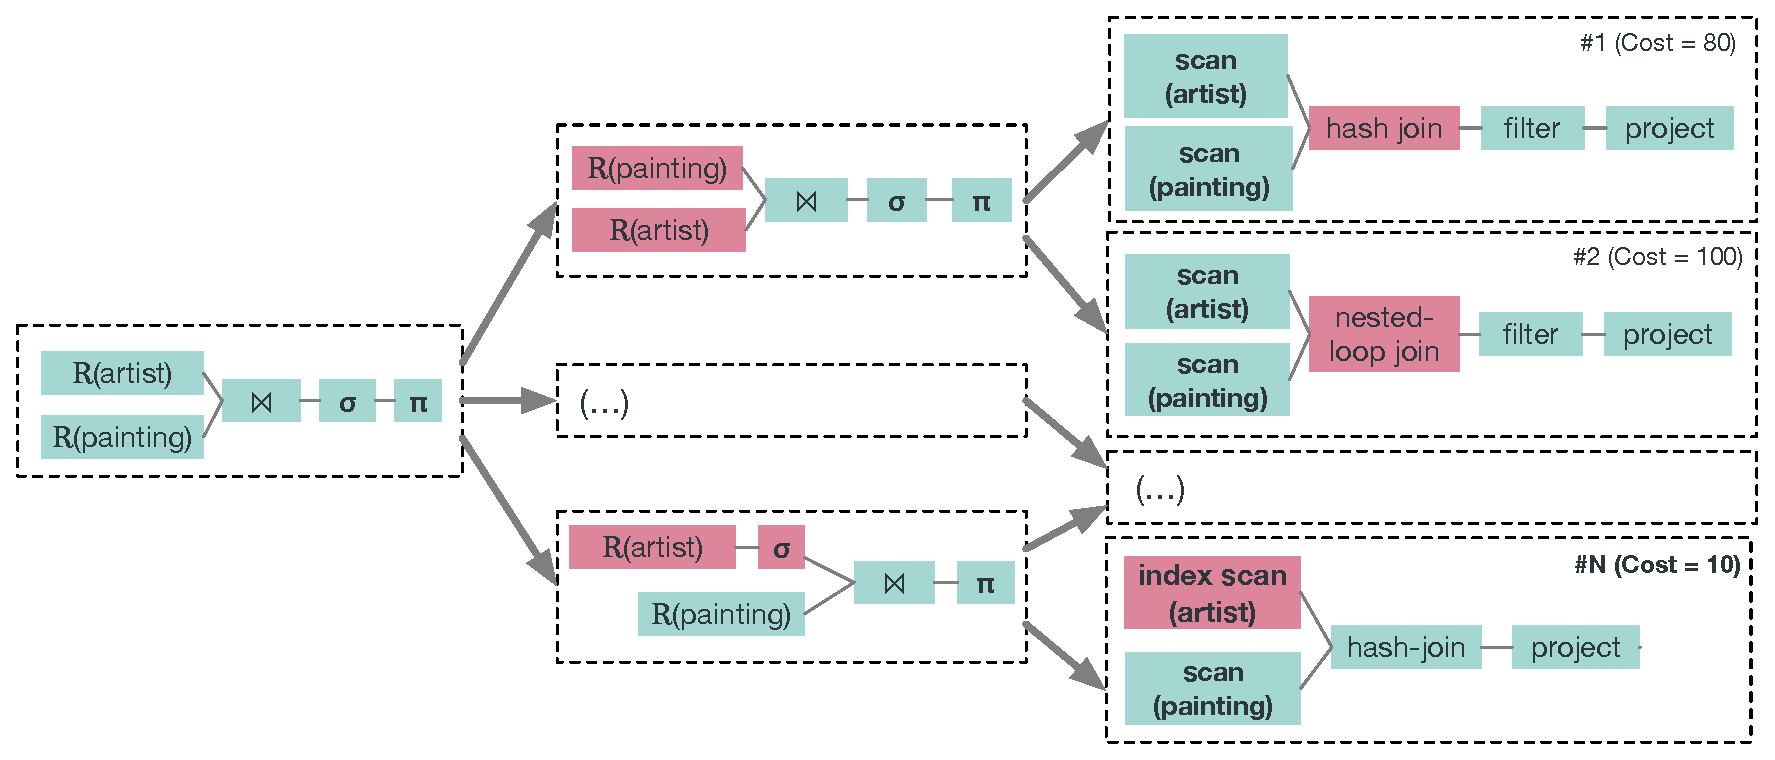
\includegraphics[width=\textwidth]{figures/query-planning.eps}
    \caption{Cost-based query planning in a \acrshort{dbms} based on \Cref{example:sql_query}. A logical input plan is transformed into different, equivalent versions and the most cost-efficient is selected.}
    \label{figure:query_planning}
\end{figure}

Early top-down approaches tried to focus on heuristic methods \cite{Jarke:1984Query}. However, the System-R paper \cite{Selinger:1979Access} published in \citeyear{Selinger:1979Access} established the idea of \emph{cost-based query optimisation} as a gold standard for \acrshort{dbms}. A cost-based query planner enumerates phyisical plans that employ different strategies and selects the one that minimises the estimated cost. Those costs may involve computation (time used on a CPU), storage access (data accessed on disk) or transmission (data transfered between nodes) required by a query \cite{Jarke:1984Query,Garcia:2009Database}. Which of those metrics are used is highly dependent on the system: In the not too distant past before the invention of \acrfull{ssd}, access to secondary storage was considered to be the defining cost and thus the main focus was to minimize disk access \cite{Garcia:2009Database}. However, for distributed databases, the moving of data between nodes has become a important factor to consider as well \cite{Bruno2013:Continuous}.

The general approach at doing cost-based query optimisation is illustrated in \Cref{figure:query_planning}. It relies on an internal representation of the query, e.g., the logical plan illustrated in \Cref{figure:query-tree} and can be summarised as follows \cite{Jarke:1984Query,Graefe:1993Volcano} \footnote{The \emph{Volcano Optimizer Generator} \cite{Graefe:1993Volcano} still builds the theoretical foundation for modern systems such as \emph{Apache Calcite}.}:

\begin{enumerate}
    \item Transformation of the logical input plan to either simplify it or to replace parts that can be covered by a specific edge-cases. This results in different, alternative logical query plans.
    \item Map the transformed, logical query plans into sequences of elementary operations with known costs by selecting specific algorithms or access patterns. This results in a (potentially larger) set of physical query plans.
    \item Estimate the total cost for the physical query plans and select the one that minimises those costs.
\end{enumerate}

Each of the aformentioned steps involve sub-steps that apply algebraic equivalence rules \cite{Garcia:2009Database}  (e.g., commutativity of operations), heuristics \cite{Garcia:2009Database,Graefe:1993Query,Swami:1989Optimization,Bruno:2010Polynomial,Tsialiamanis:2012Heuristics,} (e.g., predicate pushdown) or special rules to handle certain (edge-)cases \cite{Jarke:1984Query,Graefe:1993Query} (e.g., replace table by index scan).

A critical factor for any cost-based query optimizer is the model used for cost and cardinality estimation \cite{Jarke:1984Query,Yin:2015Robust}. Most existing systems rely on statistical modeling based on the data stored in the database \cite{Getoor:2001Selectivity,Ioannidis:2003History} as well as model for cost incurred by accessing system resources \cite{Manegold:2002Generic}. Simple statistics involve information about the number of entries in a relation or statistical moments of columns but may also rely on more complex analysis of data distribution such as histograms. This pre-hoc modeling was later complemented by taking the atained execution speed into account, which requires post-hoc analysis of an execution plan w.r.t to the cost model and created a continuous control loop between planner and execution engine \cite{Mackert:1986R}. Recent work in the field of query planning also tries to apply machine learning techniques at different levels of the cost-estimation and planning process \cite{Wu:2013Predicting,Vu:2019Deep}.

\subsection{Execution Engine}

Once a query execution plan has been selected, the execution of that plan falls to the \acrshort{dbms}'s execution engine. At a high level, every operator in the plan is typically mapped to an actual operator in a query execution pipeline that performs the necessary operations, e.g., executes a scan of a table or a specific \texttt{JOIN} algorithm. This is visualised in \Cref{figure:iterator_model}. In the resulting \emph{operator tree}, every operator functions independently, reads input, processes it and produces output that is then handed to the next operator in the tree (or to the client).

While this model is simple enough, there are a few subtle differences in how this can be implemented by a system. First, there is a distinction as to how data is being handed from operator to operator:

\begin{description}
    \item[Iterator Model] This is the model described in \cite{Graefe:1993Volcano,Graefe:1993Query} and implemented in the Cascades \cite{Graefe:1995Cascades} framework. In this model, every operator reads a single tuple, processes it and hands it to the next operator in the pipeline. Therefore, tuples are iterated one by one and handed from the leafes to the root of the operator tree.
    \item[Materialization Model] In this model, every operator reads all tuples from the input, performs its work and then forwards the entire output to the next operator in one go. This requires potentially large buffers to store intermediate results.
    \item[Batch Model] In this model, every operator reads a specific number of tuples from it inputs (a batch), processes these tuples and then forwards the batched results to the next operator. Therefore, data is processed batch by batch.
\end{description}

It must be mentioned, that even in the iterator model, some operators require intermediate materialisation (e.g. sort operators). In addition, we can distinguish between which operator initiates data exchange:

\begin{description}
    \item[Pull-based] Operators higher-up in the operator tree request the next item from the previous operator. This is the common model for disk-based systems and leads to the slowest operator in the pipeline determining execution speed.
    \item[Push-based] Operators lower in the operator tree send their results to the next operator, which has to buffer if it is not ready to process it. While potentially more efficient, this requires a buffering infrastructure.
\end{description}

The pull-based iterator model is very easy to implement, since basically, every operator just needs to implement a \texttt{next()} method that returns the next tuple (and \texttt{open()} and \texttt{close()} methods to signal start and end). The model is illustrated in \Cref{figure:iterator_model}. It is probably the most common processing model found in disk-based \acrshort{dbms}, even though, it has downsides such a poor instruction locality and overhead due to the large number of method calls \cite{Neumann:2014Compiling}. The materialization model can be beneficial for small datasets and \acrshort{oltp} queries. However, it is not a good fit for analytical workloads on large datasets, especially, if main memory is limited. The batch model is something in between the previous two and can be very when using vectorised processing and \acrshort{simd} instructions such as those provided by the \acrshort{avx} or \acrshort{sse} extensions. It is thus often employed in analytical databases such as MonetDB \cite{Idreos:2012MonetDB}.

\begin{figure}[tb]
    \centering
    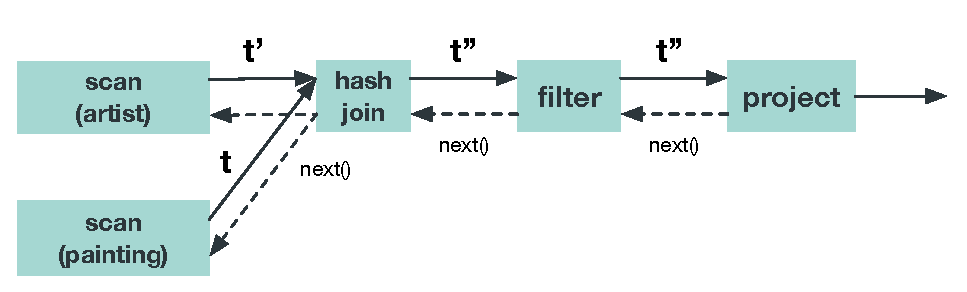
\includegraphics[width=\textwidth]{figures/iterator-model.eps}
    \caption{Illustration of the iterator model for query listed in \Cref{example:sql_query}. Every operator calls the upstream operator with \texttt{next()} to request the next tuple for processing.}
    \label{figure:iterator_model}
\end{figure}

\subsubsection{Query Parallelism}

With most computing platforms offering multiple \acrshort{cpu}s or \acrshort{cpu} cores, parallel execution of queries can provide a considerable speed-up in terms of execution time. \cite{Graefe:1993Query} distinguishes between three types of parallelism in a \acrshort{dbms}:

\begin{description}
    \item[Inter-query parallelism] refers to the parallel execution of different, independent queries (potentially from different users). At a high level, there are two approaches at achieving inter-query parallelism, namely, by mapping different queries to different system processes (e.g., PostgreSQL) or to different threads within the same process (e.g., MySQL), with the advantage of the latter being that all queries share the same memory address space.
    \item[Inter-operator parallelism] refers to the parallel execution of different operators within a query, which are then synchronised by a dedicated operator that merges the results. This is a form of \emph{intra-query parallelism}.
    \item[Intra-operator parallelism] refers to the splitting-up of the work performed by a specific operator. This typically involves the ability to parallelise based on the data, e.g., by partitioning on it and letting different operators taking care of parts of the workload.  This is also a form of \emph{intra-query parallelism}.
\end{description}

All three aspect must be handled by the query execution engine (and other component involved) and give rise to a large number of implementation details that must be considered when building a \acrshort{dbms}. For example, the challenges that arise from parallel query execution and the resulting, concurrent data access -- especially in the presence of parallel reads and writes -- are covered by the \emph{isolation} part of \acrshort{acid} and typically mitigated by a \emph{transaction manager} and \emph{concurrency control protocols}.

\subsubsection{Optimising Execution Speed}
Speeding-up query execution has been a large corpus of research at different levels and has given rise to many relevant solutions. We have already mentioned the use of specialised CPU instructions such as \acrshort{avx} or \acrshort{sse}, which is an active area of research \cite{Idreos:2012MonetDB,Polychroniou:2020VIP,Polychroniou:2019Towards,Shen:2021Using} even to the extent, that workloads are executed on a \acrshort{gpu} instead of a \acrshort{cpu} \cite{Paul:2021Database}.

An other approach used to minimise the overhead incurred by the iterator model is compilation as implemented by HyPer \cite{Neumann:2014Compiling}, which is also an active area of research \cite{Krolik:2021r3d3,Funke:2021Low}. This technique tries to compile parts of the execution plan directly into machine code, i.e., merging multiple operators into one, which increases instruction locality and allows for caching and later re-use of pre-compiled elements. The method can also be combined with vectorised execution \cite{Sompolski:2011Vectorization,Rosenfeld:2022Query}.

\subsection{Storage Manager}

At the lowest levels of any \acrshort{dbms} there is the storage manager, which orchestrates access to data on primary and secondary storage devices. Many different approaches at storage have been implemented over the years and we will simply focus on some basic concepts and refer to \cite{Petrov:2019Database} for more information on the topic. What most \acrshort{dbms} have in common is that they implement a two-level memory architecture wherin data resides on disk (which is typically slower) and in main memory (which is typically faster). The two aspects are handled by the two main components: the \emph{disk manager} and the \emph{buffer pool manager} \cite{Petrov:2019Database}.

\subsubsection{Disk Manager}
The disk manager provides access to the files that reside on disk. Most databases organsise disk access in terms of fixed-size database pages that can be read and written. Typically, the size of a page is a fixed multiple of the block-size implemented by the underlying file system and ranges between 4 to \SI{16}{\kilo\byte}.

On top of this basic page structure, different types of storage can be implemented. The classical approach is to distinguish between data and index pages and to superimpose a B-Tree structure on top of the pages \cite{Bayer:2002Organization}. Data pages contain the actual data. Index pages are required for navigating in the data and looking up records, e.g., based on a tuple identifier. There are many implementation details to be considered, such as dealing with variable-length data, dealing with data that is larger than a page, checksumming and versioning and different techniques are being applied to address these issues.

Recent work has given rise to different types of data organisation, e.g., in systems like MonetDB where data is organised in fixes size arrays called binary association tables \cite{Boncz:2008Breaking} for databases using log-structured merge trees \cite{ONeil:1996The,Sears:2012Blsm} such as JetBrains Xodus.

\subsubsection{Buffer Pool Manager}

The main objective of the buffer pool manager is to keep frequently accessed pages in memory for faster access. That is, if upper-levels of the \acrshort{dbms} require access to a given page, they request it from the buffer pool manager, which can either serve it from memory or read it from disk through the disk manager. Meanwhile, the buffer pool manager can keep track of page access and can evict or retain pages depending on usage. In addition to caching, buffer pool managers also implement different strategies for page replacement and eviction (e.g., \acrshort{fifo} or \acrshort{lru}), pre-fetching of pages depending on workloads (e.g., when scans are performed) as well as locking of pages for concurrency control.

Some \acrshort{dbms}, such as MonetDB \cite{Boncz:2008Breaking} or LMDB \cite{Henry:2019Howard}, forego the implementation of a buffer pool manager and instead rely on the \acrshort{posix} \texttt{mmap} system call \cite{Stonebraker:1981Operating}, which allows the mapping of files on disk into the address space of an application and leaves caching of pages to the operating system. While this simplifies handling of data because loading and evicition of pages must not be handled explicitly, research suggest that the use of \texttt{mmap} in a \acrshort{dbms} is far from optimal \cite{Crotty:2022Are}, and that knowledge about the database workload (e.g., random access vs. scan) allows for much more finegrained control than \texttt{mmap}.

\subsection{Common Components}

The following components are also part of a \acrshort{dbms} and are briefly described for the sake of completeness:

\begin{description}
    \item[Catalogue] The catalogue is used to persistently store and lookup information used by \acrshort{dbms} to organise the data it contains, i.e., information about units of data organisation such as tables, columns, collections, indexes as well as metadata such as statistics, transactions or locks.
    \item[Transaction] One or multiple queries processed by a \acrshort{dbms} are typically wrapped in transactions, i.e., a series of operations that should be executed together and either be committed or rolled back at the end. Often, the \acrshort{dbms} provides guarantees with respect to the execution of transactions such as \acrshort{acid} \cite{Haerder:1983principles} or \acrshort{base} \cite{Pritchett:2008Base}, e.g., assuring an all-or-nothing semantic (atomicity) for operations being executed within a transaction (the A ind \acrshort{acid}).
    \item[Transaction Managers] In order to provide the aforementioned guarantees for a transaction, the query workloads must be orchestrated across different components (e.g., disk manager, buffer pool manager, execution engine, lock manager, recovery manager). This is the main task of the transaction manager in addition to keeping track of a transaction's lifecycle.
    \item[Lock Manager] One approach to provide transaction isolation (the I in \acrshort{acid}), i.e., proper protection of the data in case different transactions access it concurrently, is the implementation \acrfull{s2pl}. This is typically provided by a lock manager, which keeps shared and exclusive locks on pages that are accessed and detects lock cycles.
    \item[Recovery Manager] Typically, databases are required to provide some form of durability with respect to the execution of a transaction. Therefore, once a transaction commits, changes are expected to be permanent (the D in \acrshort{acid}). This is guaranteed by different techniques such as write-ahead logging which allow for data reconiliation in case of a system failure (e.g., power outage). This is the main task of the recovery manager and a famous algorithm employed here is known as \acrshort{aries} \cite{Mohan:1992Aries}.
\end{description}

Obviously, some databases feature additional system components depending on concrete applications, e.g., a distribution manager for \acrshort{dbms} that provide distribution of data and processing accross multiple nodes.